\documentclass{article}
\setlength{\oddsidemargin}{0in}
\setlength{\evensidemargin}{0in}
\setlength{\textwidth}{6.5in}
\setlength{\parindent}{0in}
\setlength{\parskip}{\baselineskip}

\usepackage{amsmath,amsfonts,amssymb,geometry}
\usepackage{graphicx}
\usepackage{algorithm}
\usepackage[noend]{algpseudocode}
\usepackage{fancyhdr}
\usepackage{ulem}
\usepackage{listings}

\pagestyle{fancy}
\setlength{\headheight}{15pt}

\makeatletter
\def\BState{\State\hskip-\ALG@thistlm}
\makeatother

\begin{document}

CSCI 3104-300 Summer 2019 \hfill Problem Set 7 \\
Hoffman, Ryan \\
01/11

\hrulefill

\vspace{-3mm}
\begin{enumerate}
	% HARD PROBLEM
    \item (30 points) Grog gives you the following unweighted graph and asks you to construct a weight function $w$ on the edges, 
    using positive integer weights only, such that the following conditions are true regarding minimum spanning trees (MST) and 
    single-source shortest path trees (SSSP):
	    \begin{itemize}
	        \itemsep-0.1pt
	        \item The MST is distinct from any of the seven SSSP trees.
	        \item The order in which Jarn\'ik/Prim's algorithm adds the safe edges is different from the order in which Kruskal's algorithm adds them.
	    \end{itemize}
    Justify your solution by (i) giving the edges weights, (ii) showing the corresponding MST and all the SSSP trees, and 
    (iii) giving the order in which edges are added by each of the two algorithms.
    % ----- FIGURE 1 : unweighted_graph.png -----
    \begin{figure}[h!]
    \begin{center}
    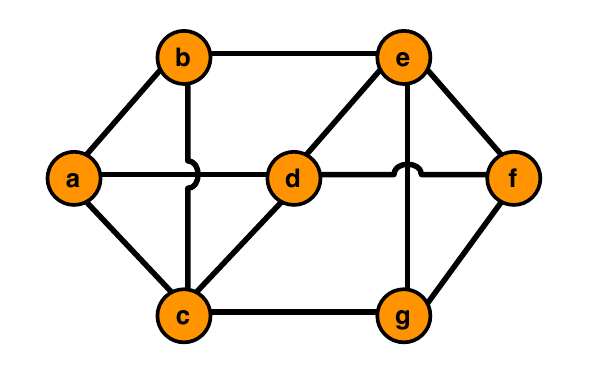
\includegraphics[scale=0.7]{unweighted_graph.png} 
    \end{center}
    \end{figure}
    % ----------
    \par
    \pagebreak
    \textbf{Solution:}\par
        \begin{figure}[h!]
        \begin{center}
        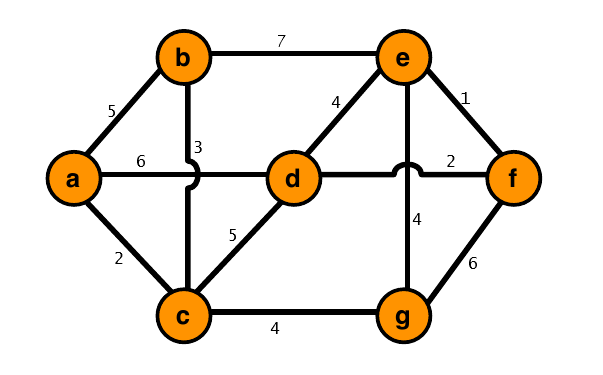
\includegraphics[scale=0.5]{weighted_graph.png} 
        \end{center}
        \end{figure}
        \begin{figure}[h!]
        \begin{center}
        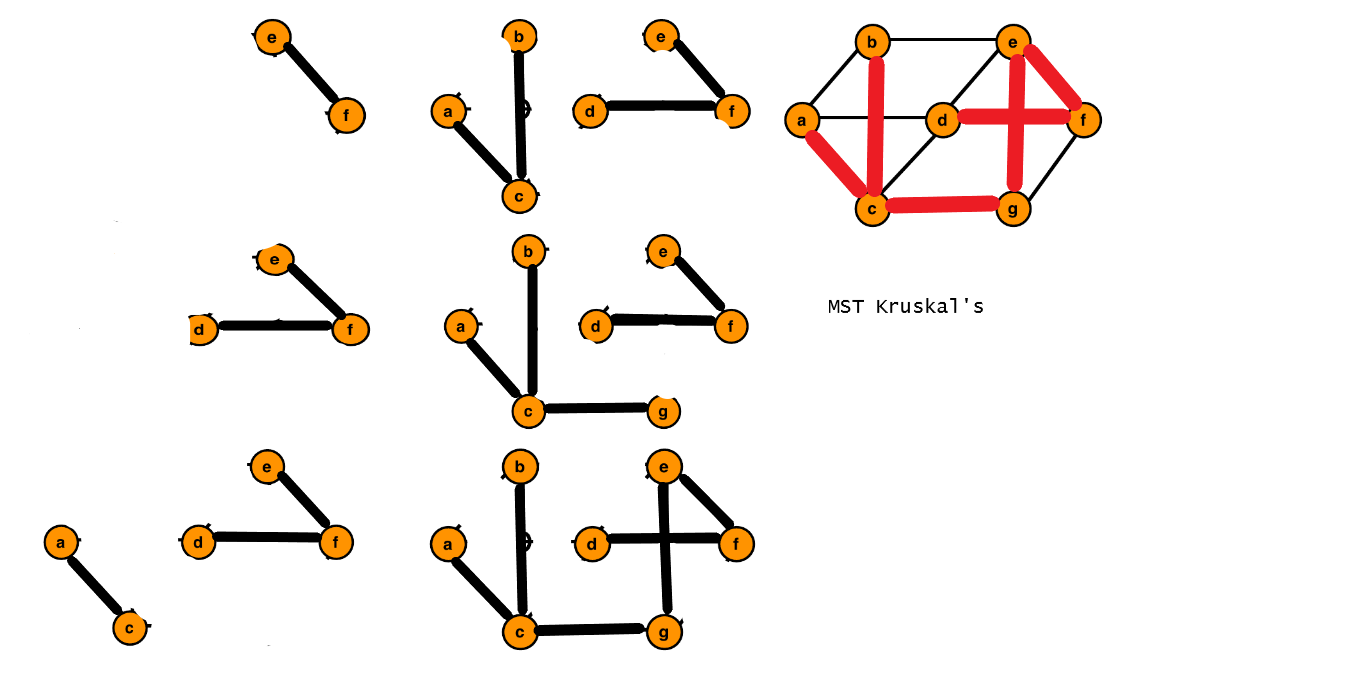
\includegraphics[scale=0.5]{mst_kruskal.png} 
        \end{center}
        \end{figure}
        \begin{figure}[h!]
        \begin{center}
        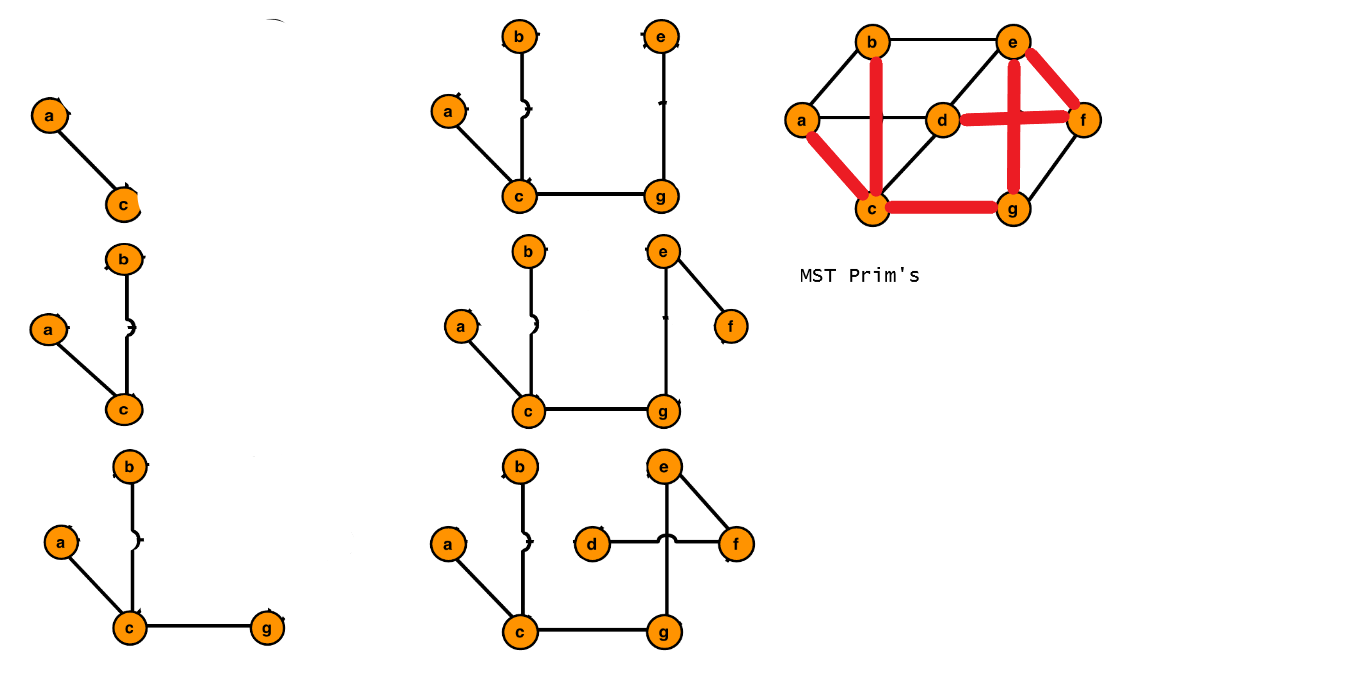
\includegraphics[scale=0.5]{mst_prim.png} 
        \end{center}
        \end{figure}
        \begin{figure}[h!]
        \begin{center}
        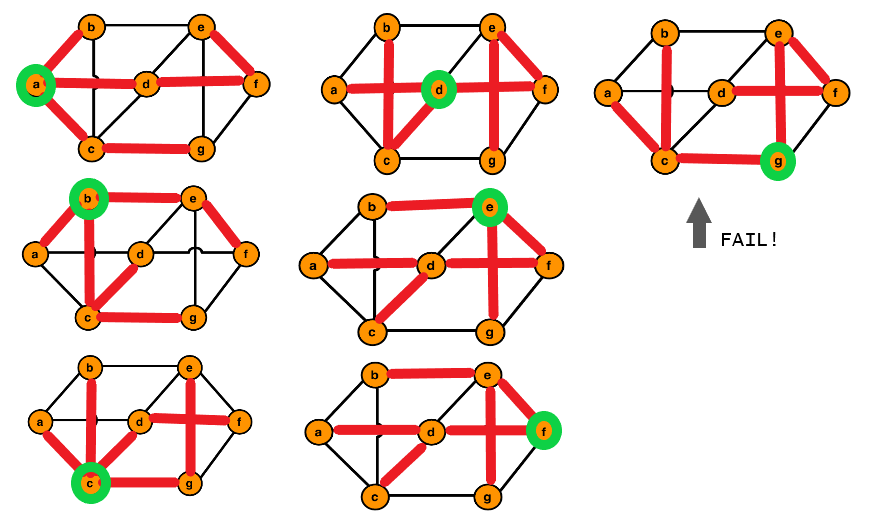
\includegraphics[scale=0.5]{Dijkstras.png} 
        \end{center}
        \end{figure}
        \par
    \pagebreak

	% CURRENCY ARBITRAGE
    \item (25 points) Harry and Shadow think they have come up with a way to get rich by exploiting the ore market.
	    \begin{enumerate}
            \item When given $R$ and $\alpha$, give an efficient algorithm that can determine if an arbitrage opportunity exists. 
            Analyze the running time of your algorithm.
	        Thormund's hint:\ It is possible to solve this problem in $O(n^{3})$.\par
            \textbf{Solution:}\par
                Using Bellman-Ford to determine if a negative-weight cycle exists. To do this, however, we need to introduce
                a vertex $s$, with weight $0$ from $s$ to all vertices. This way, we can detect a negative cycle if it exists. We also need a weight function that takes into
                account the given transaction cost $\alpha$.\par
                Here is the weight function: \par
                $$w(v_i, v_j) = \lg \frac{1}{R[i, j]\alpha }$$ \par 
                $$= -\lg R[i, j]\alpha $$\par
                This gives us a directed negative-weighted graph to work with\cite{dailycodingproblem}.\par
                Now, since Bellman-Ford returns \textit{True} if no negative-weight cycle exists and \textit{False} otherwise, we just need to invert the result.\par
                Analysis:\par
                To create the directed, negative-weighted graph is $\Theta(n^2)$\par
                Running Bellman-Ford in the above algorithm is $O(n^{3})$.\cite{cs.princeton}
            \item For an arbitrary $R$, explain how varying $\alpha$ changes the set of arbitrage opportunities that exist and that your 
            algorithm might identify.\par
            \textbf{Solution:}\par
            Variations on the transaction cost, $\alpha$, affects the no-arbitrage condition by creating an area (or region) where arbitrage is not profitable.\cite{semantic}
        \end{enumerate}        
    \pagebreak
	
    % PROGRAMMING PROBLEM
    \item 

    \begin{enumerate}

    \item \textbf{Solution:}\par
        Not able to produce a solution.
    \item \textbf{Solution:}\par
        Not able to produce a solution.
    \item 
        \begin{enumerate}
            \item Grids.        
            \begin{figure}[H]
            \begin{center}
            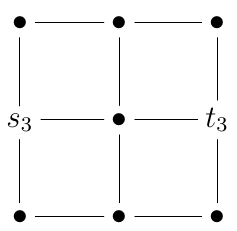
\includegraphics[scale=0.9]{grid.png} 
            \end{center}
            \end{figure}\par
            \textbf{Solution:}\par
                Not able to produce a solution.
            \item Trees.
            \begin{figure}[H]
            \begin{center}
            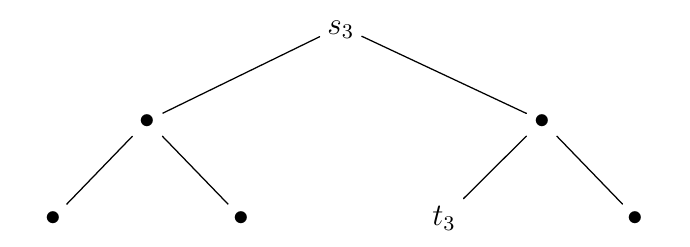
\includegraphics[scale=0.6]{tree.png} 
            \end{center}
            \end{figure}\par
            \textbf{Solution:}\par
                Not able to produce a solution.
            \item Random graphs.\par
            \textbf{Solution:}\par
                Not able to produce a solution.
        \end{enumerate}
    \end{enumerate}
\end{enumerate}
\pagebreak
\begin{thebibliography}{999}

    \bibitem{dailycodingproblem}
        https://www.dailycodingproblem.com/blog/how-to-find-arbitrage-opportunities-in-python/
    \bibitem{cs.princeton}
        http://www.cs.princeton.edu/courses/archive/spring06/cos226/lectures/shortest-path.pdf
    \bibitem{semantic}
    https://pdfs.semanticscholar.org/7285/359f5cf6cac25a54c4b2126a090352bf1fe4.pdf
    \end{thebibliography}
\end{document}
